\documentclass{article}

\usepackage{arxiv}

\usepackage[utf8]{inputenc} % allow utf-8 input
\usepackage[T1]{fontenc}    % use 8-bit T1 fonts
\usepackage{hyperref}       % hyperlinks
\usepackage{url}            % simple URL typesetting
\usepackage{booktabs}       % professional-quality tables
\usepackage{amsfonts}       % blackboard math symbols
\usepackage{nicefrac}       % compact symbols for 1/2, etc.
\usepackage{microtype}      % microtypography
\usepackage{cleveref}       % smart cross-referencing
\usepackage{lipsum}         % Can be removed after putting your text content
\usepackage{graphicx}
\usepackage{natbib}
\usepackage{doi}
\usepackage[portuguese]{babel}
\usepackage{caption}
\usepackage{braket}


\graphicspath{ {../images/} }

\title{Quantum Oracles - Como transformar problemas clássicos em quânticos}

\date{}


\author{ \href{https://orcid.org/0009-0008-9134-5974}{
\includegraphics[scale=0.06]{orcid.pdf}\hspace{1mm}Alexandre Silva}\\
	Ciências da Computação\\
	UNIVEM - Centro Universitário Eurípides de Marília\\
}



\renewcommand{\headeright}{}
\renewcommand{\undertitle}{}
\renewcommand{\shorttitle}{}


\hypersetup{
pdftitle={Quantum Oracles - Como transformar problemas classicos em quanticos},
pdfsubject={quantum computing, computer science, ciencias da computacao, computacao quantica, algoritmos, algorithms},
pdfauthor={Alexandre Silva},
pdfkeywords={quantum oracles, quantum, quantum computing, algoritmos, algorithms},
}

\begin{document}
\maketitle

\begin{abstract}
	
\end{abstract}


\section{Introdução}
Hoje, não é difícil ver alguém falando sobre computação quântica e como essas máquinas vão mudar o futuro. Contudo, muitas dessas frases acabam se levando por extrapolações e/ou usos indevidos de ficção. Neste artigo, mostrarei que nem tudo é possível ser feito com um computador quântico atual, assim como existem pequenas áreas que se beneficiam ao máximo dessa nova tecnologia.\\
Para esse feito, serão mostrado alguns testes feitos usando o \href{https://www.ibm.com/quantum/qiskit}{qiskit}, um framework open source da IBM para computação quântica, além de alguns resultados obtidos após executar os algoritmos em simuladores e máquinas reais, assim como seus relativos em computação clássica. Algoritmos dos quais tomam proveito dos quantum oracles, modelos ideias de função que não ajudam a descrever o algoritmo matematicamente, também tomam proveito de alguns efeitos quânticos, como superposição e interferência, para se sobressair à algumas estratégias clássicas.\\
Com isso, o projeto foi desenvolvido em cima de cinco pequenos problemas, sendo eles: conversão de milhas para quilômetros, torre de Hanoi, explorador de arquivos, Buckshot Roulette e QRAM. Todas as implementações e materiais utilizados podem ser encontrados \href{https://github.com/Dpbm/scientific-initiation-1-quantum-oracles}{nesse repositório do GitHub}.


\section{Início do projeto}
Para dar início a pesquisa, foi necessário entender quais os tipos de oracles existem e como eles podem ser usados.\\
Em computação clássica, temos as Oracle Machines, as quais são maquinas de Turing, das quais implementam alguma função em seu interior, e ao ser chamado/invocado o resultado correto é retornado em tempo constante $O(1)$, podendo ser vista como uma caixa preta, abstraindo completamente o seu funcionamento. Devido a essa definição, as OMs são ideias matemáticos, sendo assim usados apenas para formalismo matemático.\\
Contudo em computação quântica, podemos de fato implementar certos modelos de Oracles e adiciona-los a um circuito maior, executando certas funções como: encoding de dados, aplicação de $f(x)$, abstração de partes do circuito, etc.

\subsection{Tipos de Oracles}

\subsubsection{Phase Oracle}
Um dos primeiros tipos de Oracles usados para a criação de algoritmos como os de: \href{https://en.wikipedia.org/wiki/Grover%27s_algorithm}{Grover} e \href{https://en.wikipedia.org/wiki/Deutsch%E2%80%93Jozsa_algorithm}{Deutsch–Jozsa}; é comummente conhecido como \emph{Phase Oracle}.\\
Tal dispositivo, é usado para atribuir uma fase ao circuito, sendo muito usado para configurar valores, explorar a interferência ou se aproveitar de outros efeitos como o \textit{Phase Kickback}. Matematicamente poderiamos descrever ele da seguinte forma: $\ket{x}\ket{-} \to (-1)^{f(x)}\ket{x}\ket{-}$, do qual $\ket{x}$ é a entrada do oracle e $\ket{-}$ é a ancilla que prove a fase.

\begin{center}
	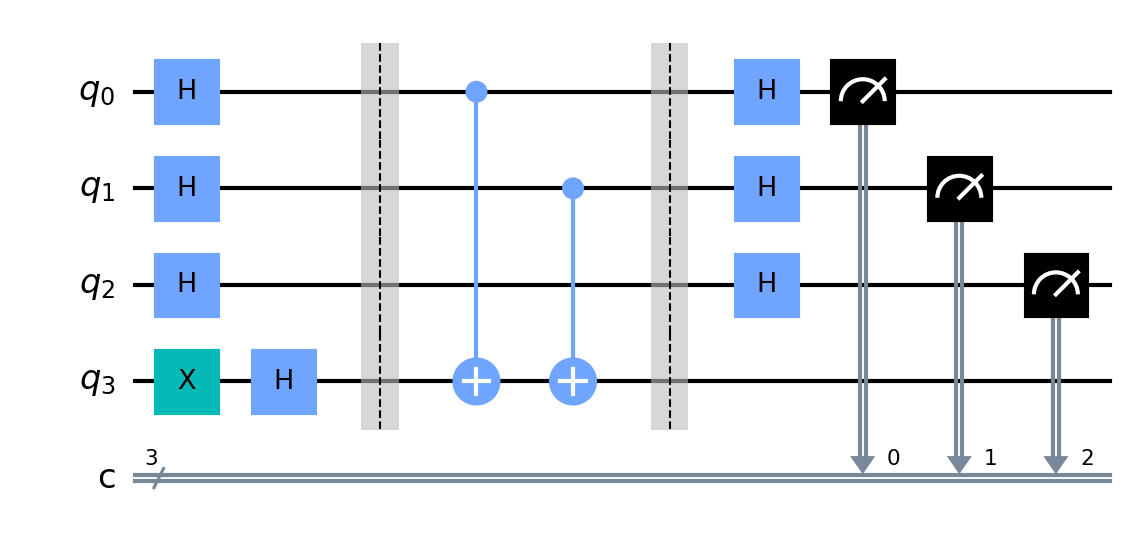
\includegraphics[scale=0.3]{phase_oracle_1.png}
	\captionof{figure}{Exemplo de phase oracle usado para o algoritmo de Deutsch–Jozsa}
	\label{fig:phase-oracle-1}
\end{center}

No exemplo acima, utilizamos o \textit{Phase Kickback} para adicionar uma fase nos qubits 0 e 1, transformando seus estados de $\ket{+}$ para $\ket{-}$, fazendo com que ao serem colapsados o resultado $\ket{1}$ apareça na saída.\\

É possível também criar um phase oracle removendo o qubit adicional (nesse exemplo o Q3), uma vez que podemos utilizar outros gates para introduzir a fase e manter ainda natureza unitária.

\begin{center}
	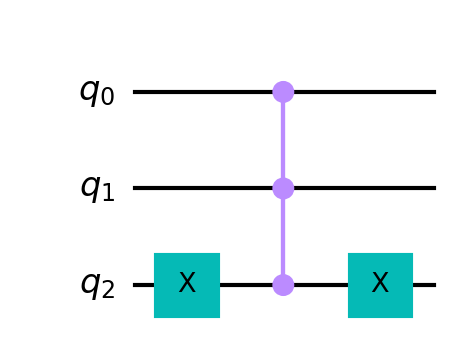
\includegraphics[scale=0.3]{phase_oracle_2.png}
	\captionof{figure}{Exemplo fase Oracle sem a Ancilla}
	\label{fig:phase-oracle-2}
\end{center}


Dessa vez, utilizamos o $MCP$ gate para adicionar uma fase global $\pi$ e dois gates $X$ para dizer quais qubits queremos q tenham o valor 0, codificando assim o valor $011$ ou $3$ na base decimal.

\begin{center}
	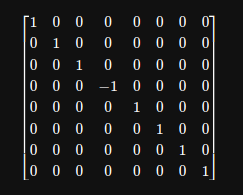
\includegraphics[scale=0.5]{phase_oracle_unitary.png}
	\captionof{figure}{Matriz unitária do Phase oracle}
	\label{fig:phase-oracle-unitary}
\end{center}

É possível verificar então que ao criarmos esse circuito, matemos a matriz identidade e adicionamos a fase $-1$ no valor da coluna relativa ao $011$. \\
Essa versão pode ser considerada como um minimal oracle, uma vez que a própria função interna se mantém unitária, sem a necessidade de ancilla.


\subsection{Boolean Oracle}

O Boolean oracle, por sua vez, representa uma função booleana, sem qualquer adição de fases.\\
Nesse caso, $\ket{x}$ representa a entrada do oracle e $\ket{y}$ represetam os qubits auxiliares que receberam a resposta, $\ket{x}\ket{y} \to \ket{x}\ket{y \oplus f(x)}$.

\subsection{Minimal oracle}

Como já citado anteriormente, o minimal oracle possui uma função que em sua essência é unitária, não requerendo qubits adicionais $\ket{x} \to \ket{f(x)}$.

\begin{center}
	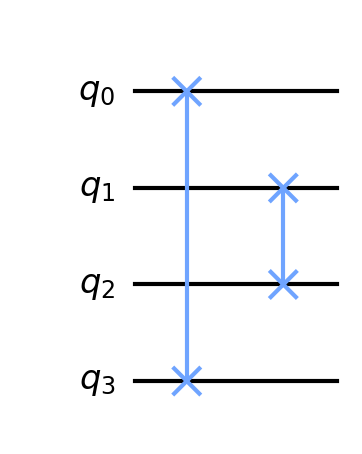
\includegraphics[scale=0.3]{minimal-oracle.png}
	\captionof{figure}{Exemplo de minimal oracle}
	\label{fig:minimal-oracle}
\end{center}

Lembrando que este pode também adicionar fases ao circuito.

\subsection{Simon's Oracle}

O Oracle de Simon, é uma instância do Boolean Oracle. Neste visamos encontrar os períodos da função implementada, ou seja, dado $x$ e $f(x) = y$ existe ao menos uma função em que $f(y) = x$ ?


\begin{center}
	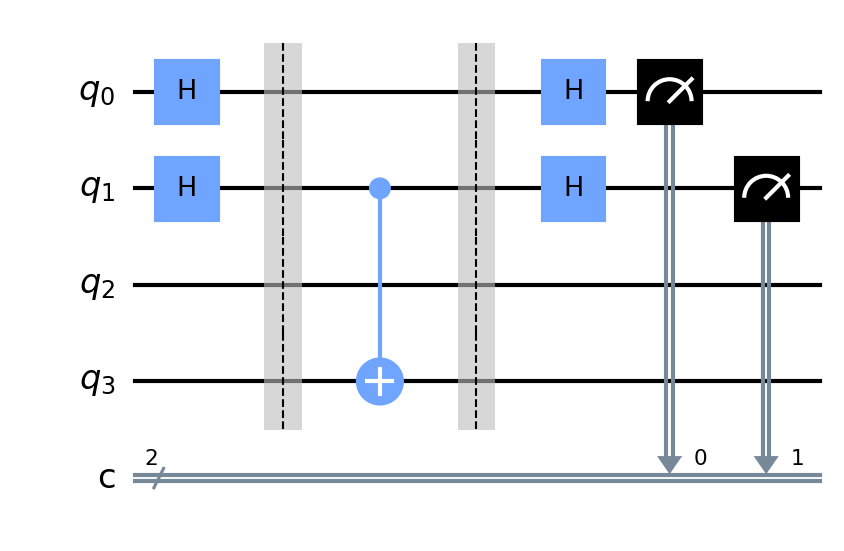
\includegraphics[scale=0.3]{simons.png}
	\captionof{figure}{Exemplo do algoritmo de Simon}
	\label{fig:simons-oracle}
\end{center}

Nesse algoritmo, configuramos uma chave $s$ dentro do oracle, e ao executar o algoritmo temos os possíveis períodos da função, sendo necessário rotinas de pós processamento para identificar o valor correto.

\subsection{QFT(Quantum Fourier Transformation) Oracle}

Por fim, o Oracle QFT aplica a versão quântica da transformada de Fourier, projetando os valores de entrada na base $X$ (também conhecido como base de Fourier).


\begin{center}
	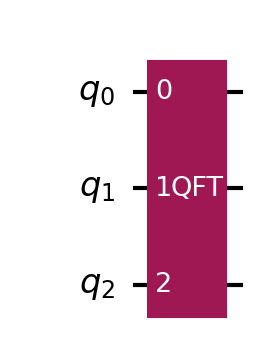
\includegraphics[scale=0.4]{QFT_1.png}
	\captionof{figure}{Exemplo do algoritmo de QFT}
	\label{fig:QFT}
\end{center}

\begin{center}
	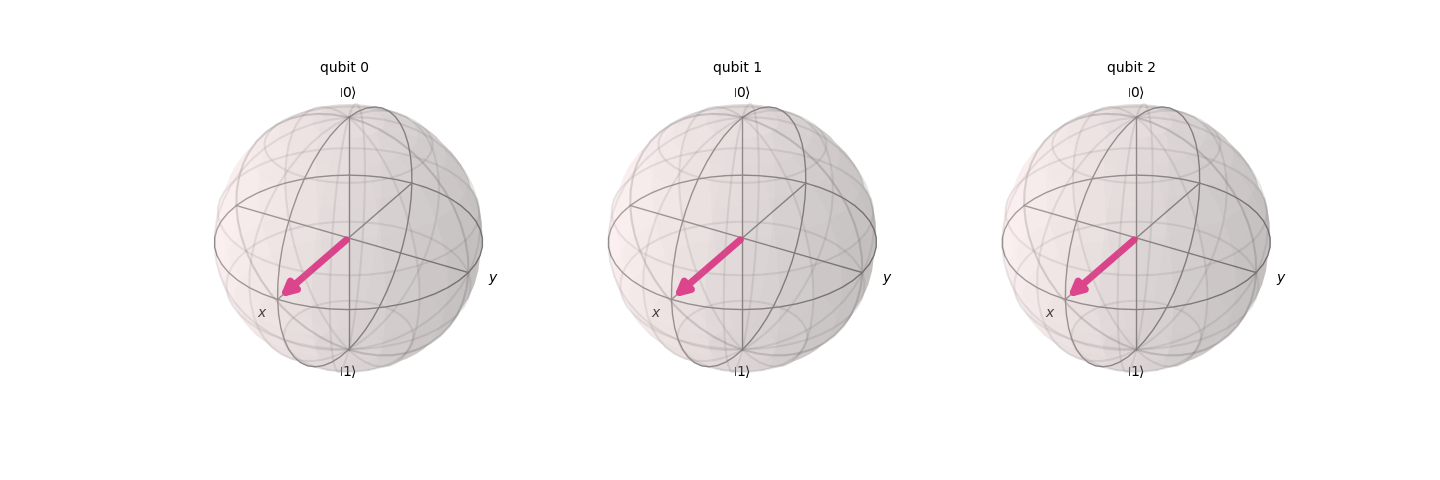
\includegraphics[scale=0.3]{QFT_1_bloch.png}
	\captionof{figure}{Valores mapeados na base de Fourier}
	\label{fig:QFT-bloch}
\end{center}


\section{Desenvolvimento}

\subsection{File Explorer}
\subsection{Miles to Kilometers}
\subsection{Hanoi Tower}
\subsection{Buckshot Roulette}
\subsection{QRAM}

\begin{center}
\end{center}


\bibliographystyle{unsrtnat}
\bibliography{references}  


\end{document}
